\chapter{Experimental Results}

In this chapter, we present the results that we acquired while testing our method. We tested our method using real datasets collected from 1000 Genome Project and Turkish Genome Project. Since there is no validated results for paralog genes, we compare our results with the results of mrCaNaVaR \cite{alkan2009personalized}, a tool to discover structural variations in duplicated regions. mrCaNaVaR, like our method, was based on read depth and it was designed to determine absolute copy numbers in duplicated regions \cite{kahveci2018whole}. However it requires a sequence alignment file with multiple read mapping, such as mrFAST \cite{alkan2009personalized}.


\section{Datasets}
We tested our method with two human genomes: NA12878 from 1000 Genome project and 42S291210 from Turkish Genome project. In general, 30X sequencing coverage is adequate for clinical-level research \cite{shevchenko2016clinical}. Therefore we picked one genome (NA12878) as an example of a human genome sequence with a high coverage (43x) and another genome (42S291210) as an example of relatively low coverage genome (20x).

\section{Results}
In this section, the results of mrCaNaVaR and our method are compared via several plots. The results include absolute copy numbers of paralog genes (i.e. genes overlapping with segmental duplications). It is not expected the results to match perfectly, however, they should show some level of consistency. We measure the consistency as overlapping percentages. The overlapping percentages are the ratio of absolute copy numbers. For example, the \%90 or more overlapping are calculated  as; $$\frac{90}{100} < \frac{CNV_{our\_method}}{CNV_{mrCaNaVaR}} < \frac{100}{90} $$.


Table \ref{overlapTable} shows the statistics on the level of consistency between our method and mrCaNaVaR. 
For NA12878, among 1205 genes for which an absolute copy number is computed by both method, 98 genes show \%90 overlapping and for 42S291210, among 1052 genes, 91 genes show \%90 overlapping.

\begin{table}[!htbp]
    \centering
    \begin{tabular}{lll}
    \hline
    \textbf{Overlap}             & \textbf{NA12878} & \textbf{42S291210}   \\ \hline
    \textbf{\%90 or more} & 98      & 91   \\
    \textbf{\%75 or more} & 266     & 219  \\
    \textbf{\%50 or more} & 625     & 487  \\
    \textbf{\%25 or more} & 961      & 769   \\ \hline
    \textbf{Total}        & 1205    & 1052 \\ \hline
    \end{tabular}
    \caption{Comparison of our method and mrCaNaVar.}
    \label{overlapTable}
\end{table}


\begin{sidewaysfigure}[ht]
    \centering
    \subfloat[NA12878]{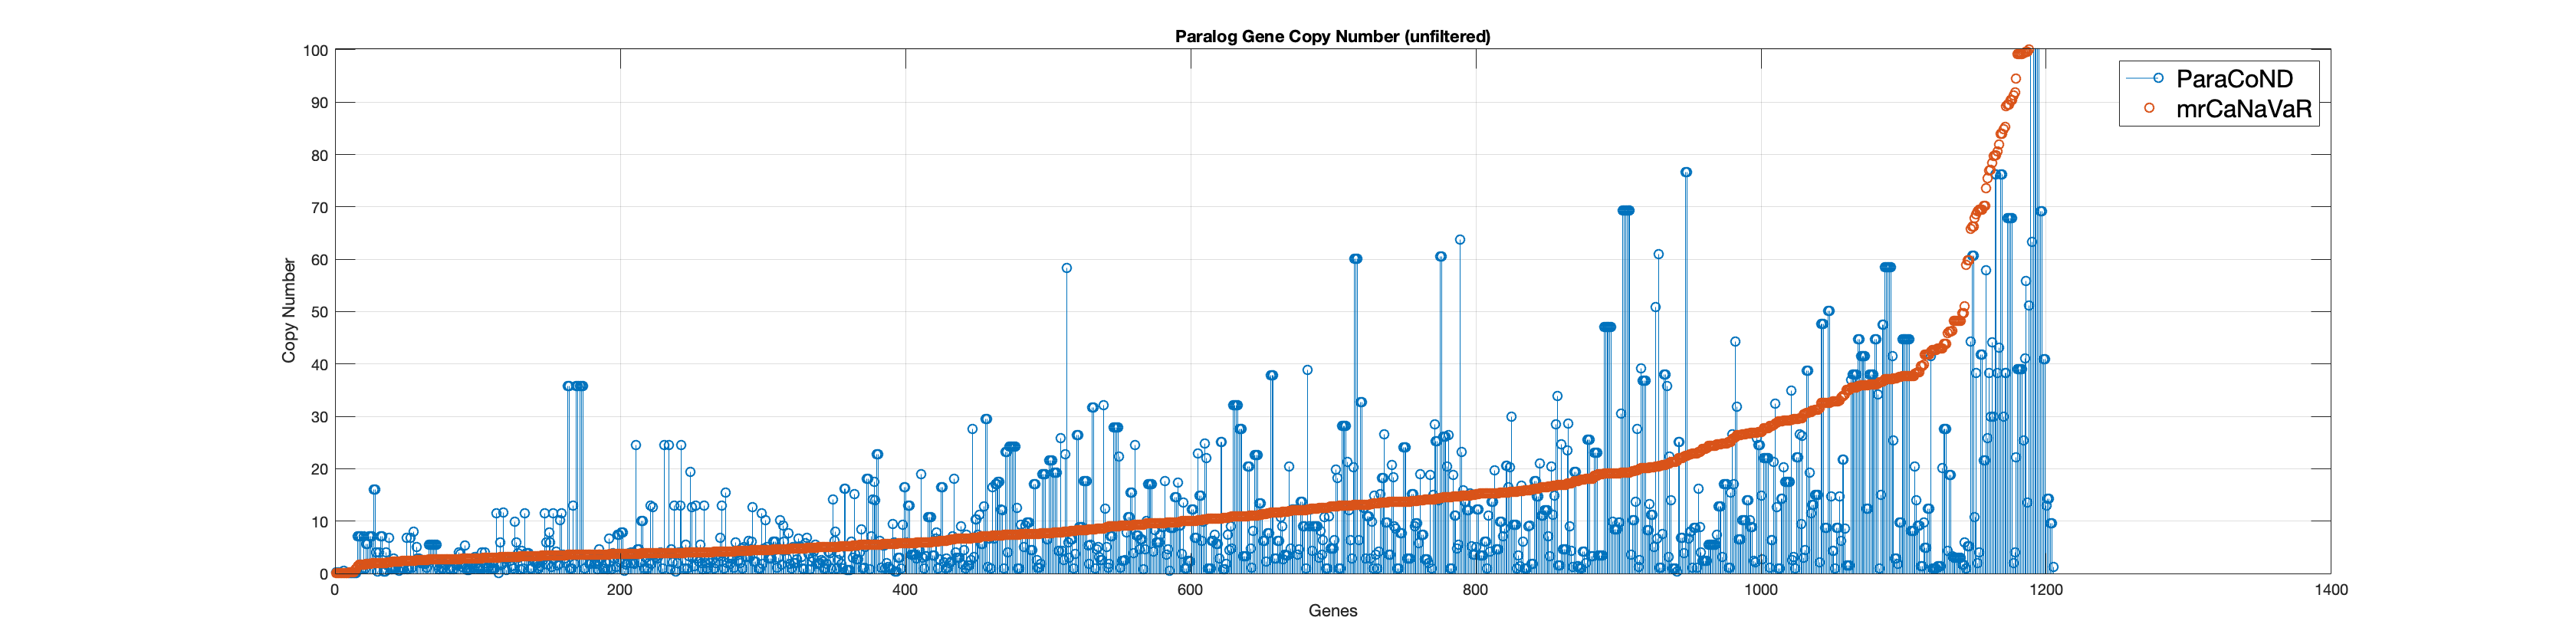
\includegraphics[scale=0.18]{images/na12878/figure1.png}\label{na12878unfiltered}}\quad
    \subfloat[42S291210]{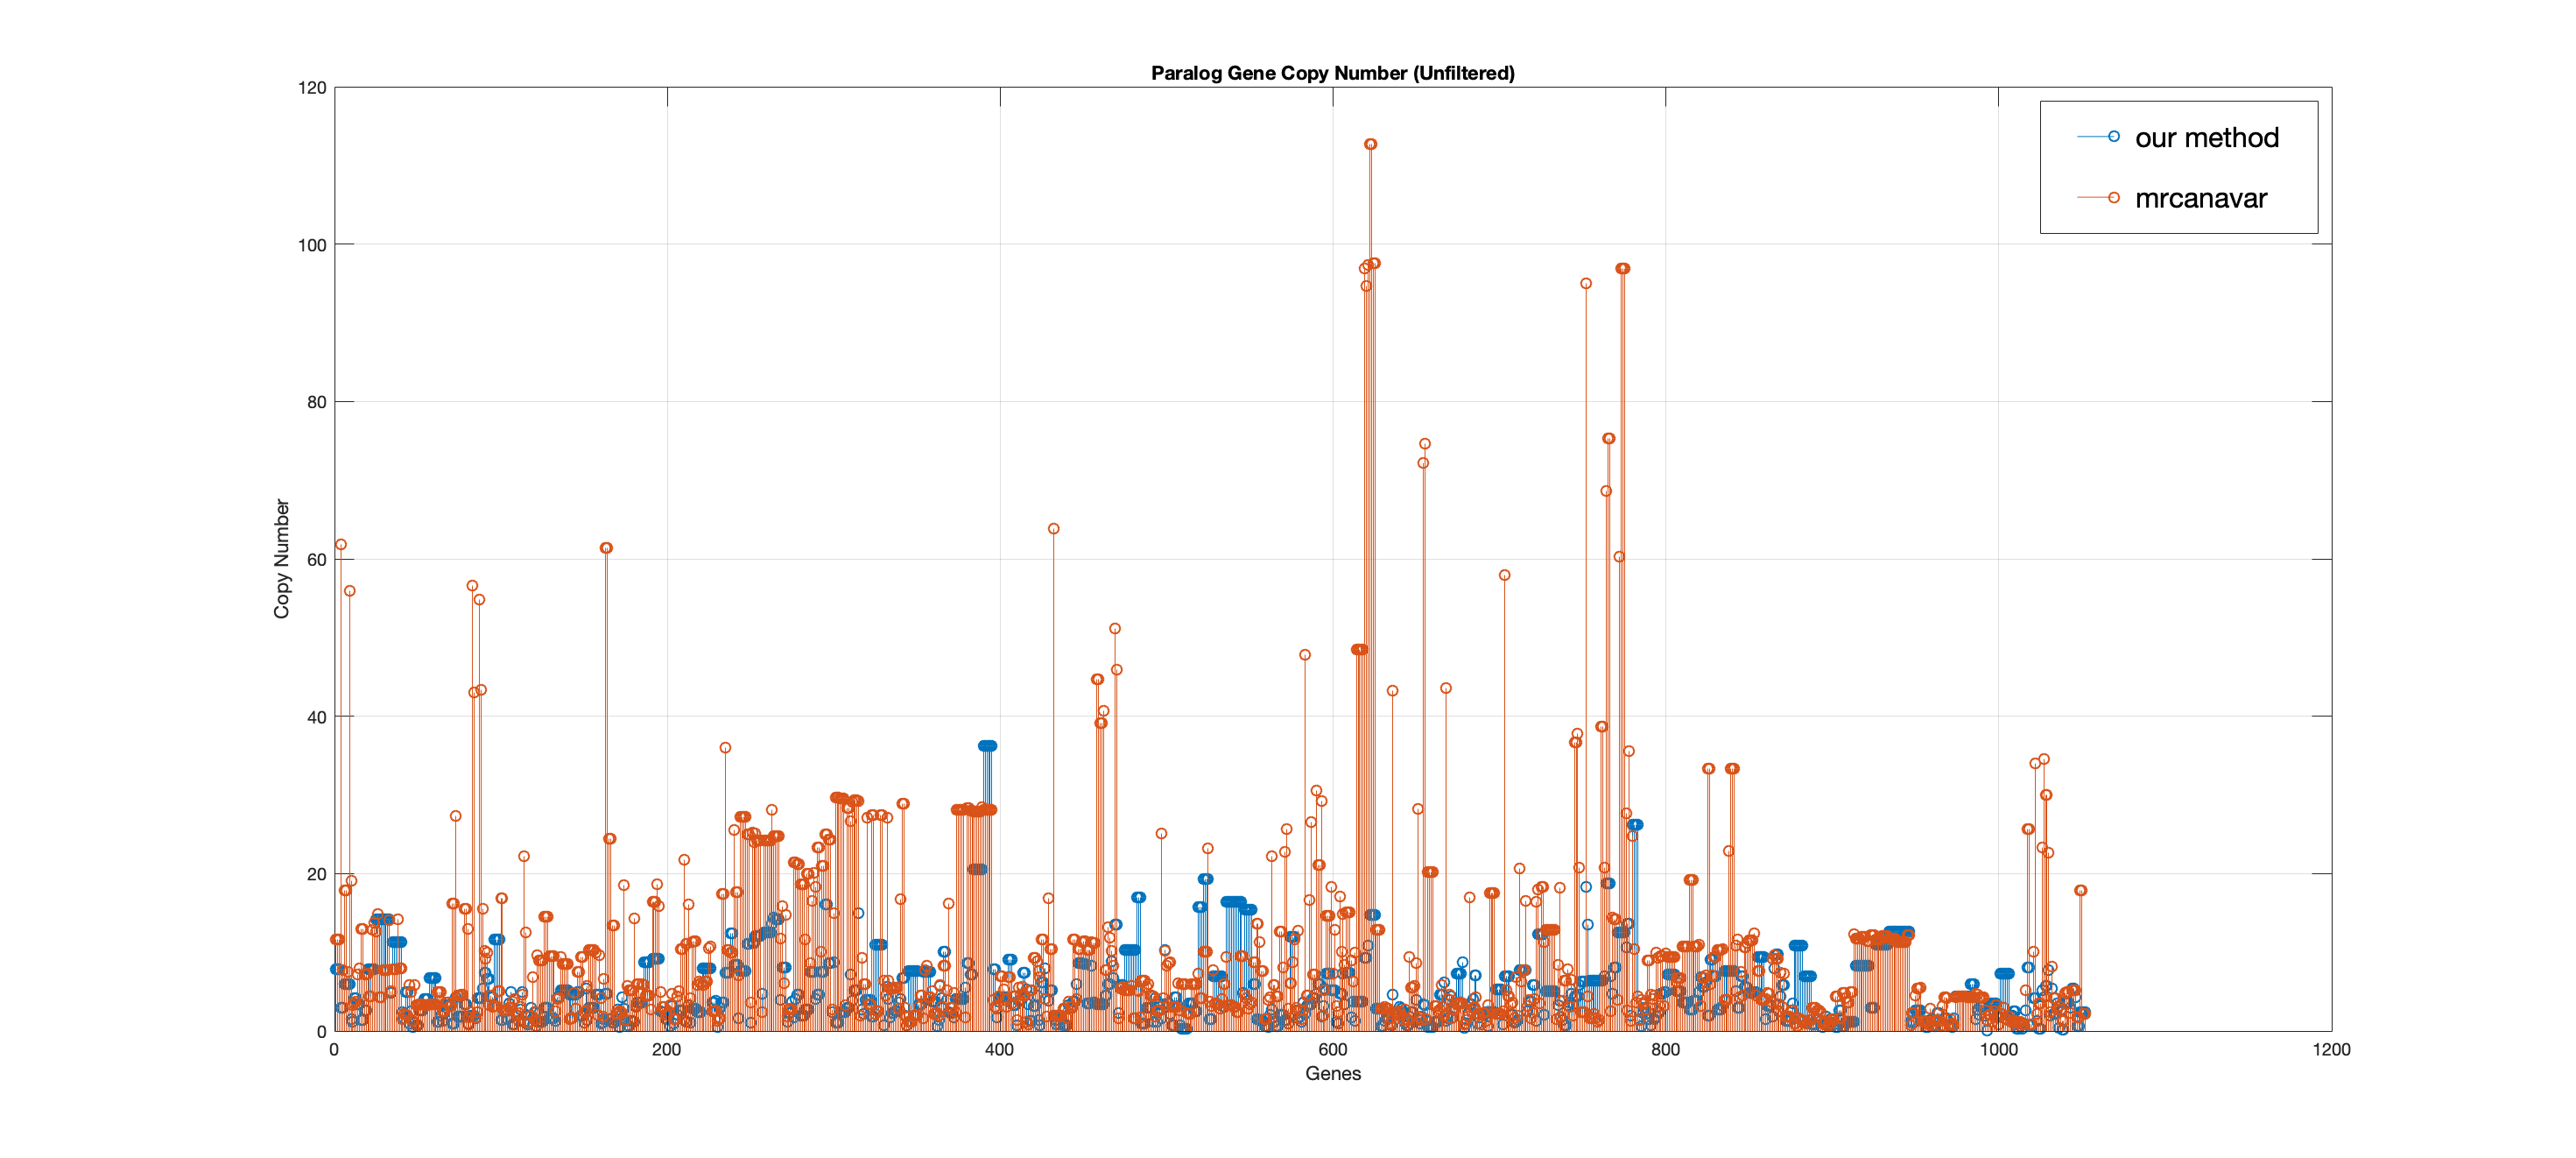
\includegraphics[scale=0.20]{images/42/figure1.png}\label{42unfiltered}}
    \caption{Absolute copy numbers of genes overlapping with segmental duplications}
    \label{unfiltered}
\end{sidewaysfigure}

\begin{figure}
    \centering
    \subfloat[NA12878]{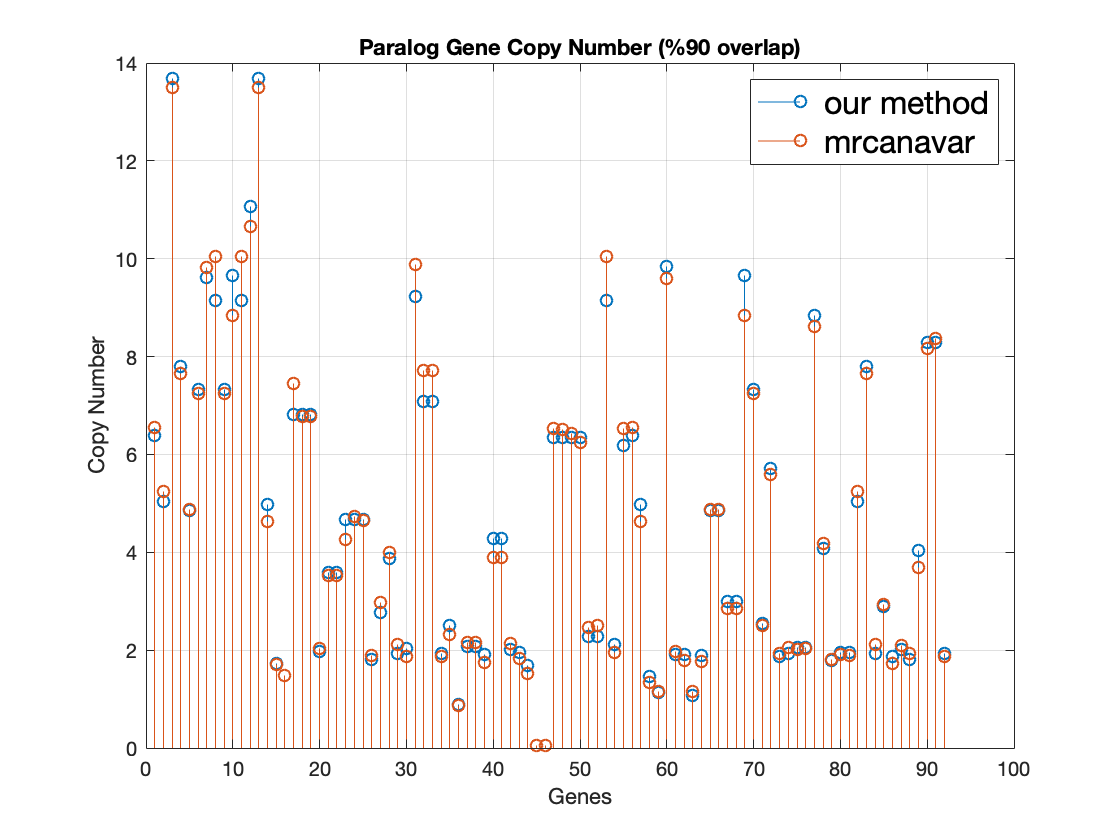
\includegraphics[scale=0.30]{images/na12878/figure2.png}\label{na12878overlap90}}\quad
    \subfloat[42S291210]{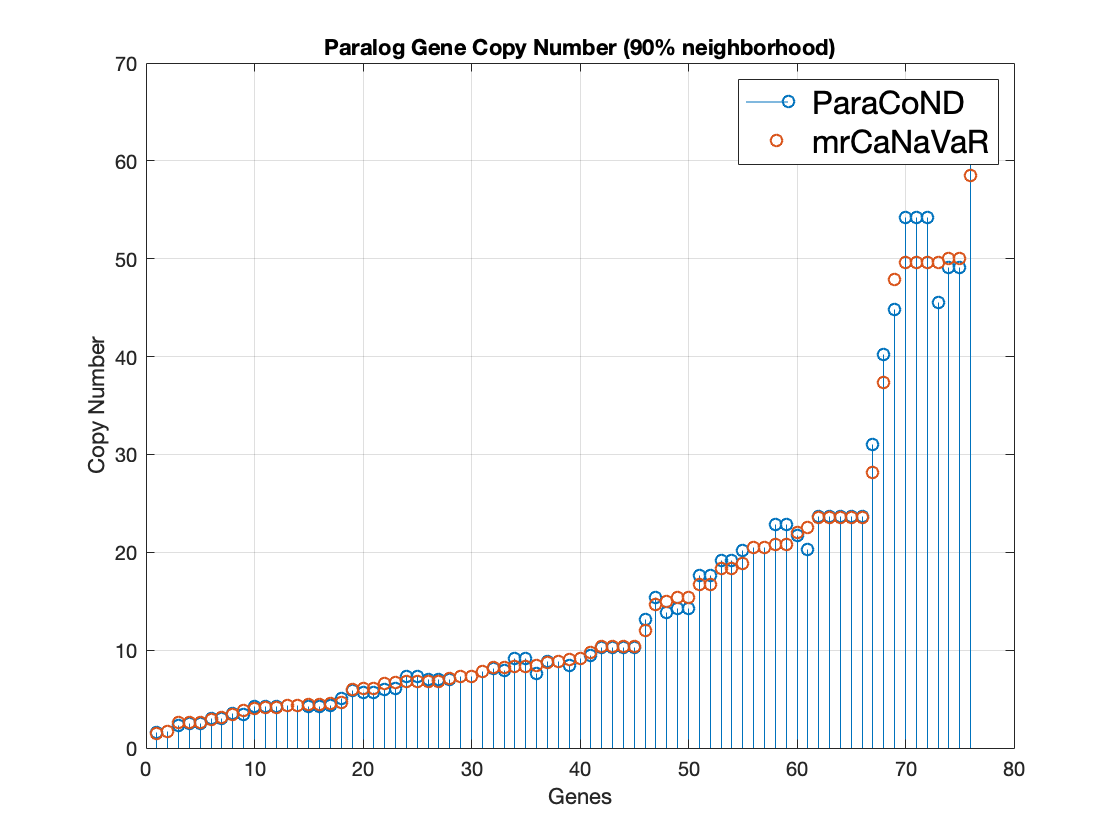
\includegraphics[scale=0.30]{images/42/figure2.png}\label{42overlap90}}
    \caption{Absolute copy numbers of genes showing \%90 overlapping by both methods}
    \label{overlap90}
\end{figure}

\begin{sidewaysfigure}[ht]
    \centering
    \subfloat[NA12878]{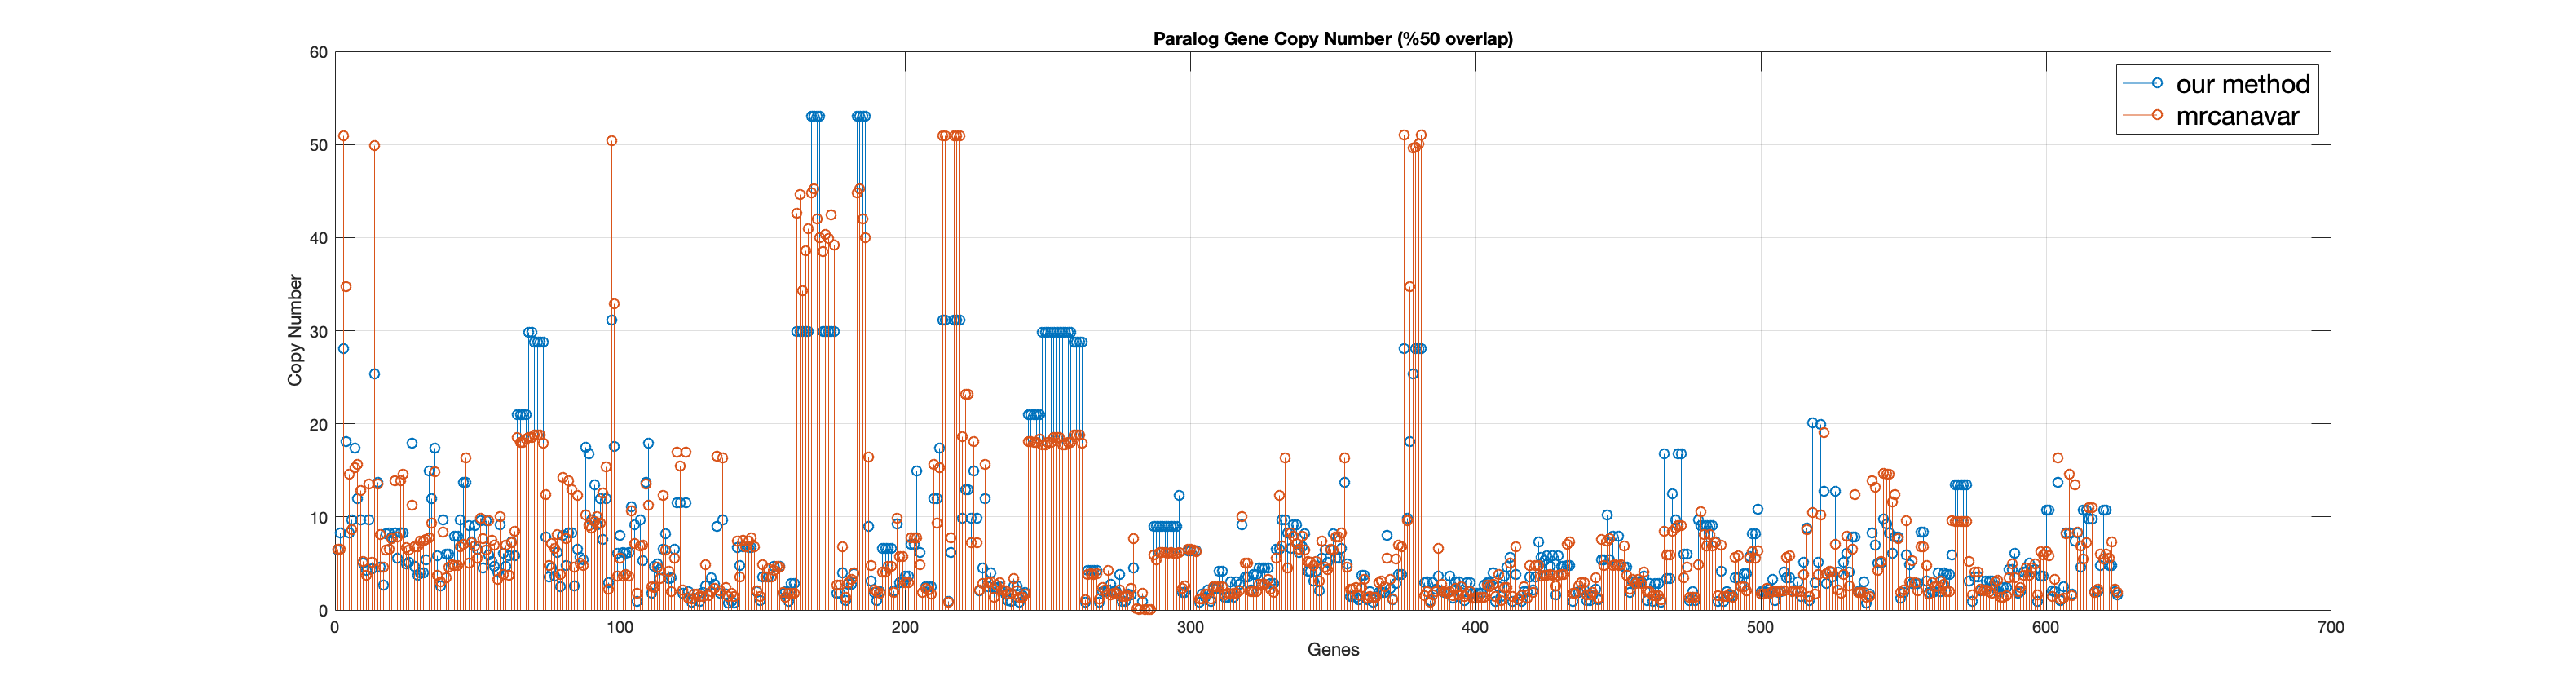
\includegraphics[scale=0.18]{images/na12878/figure3.png}\label{na12878overlap50}}\quad
    \subfloat[42S291210]{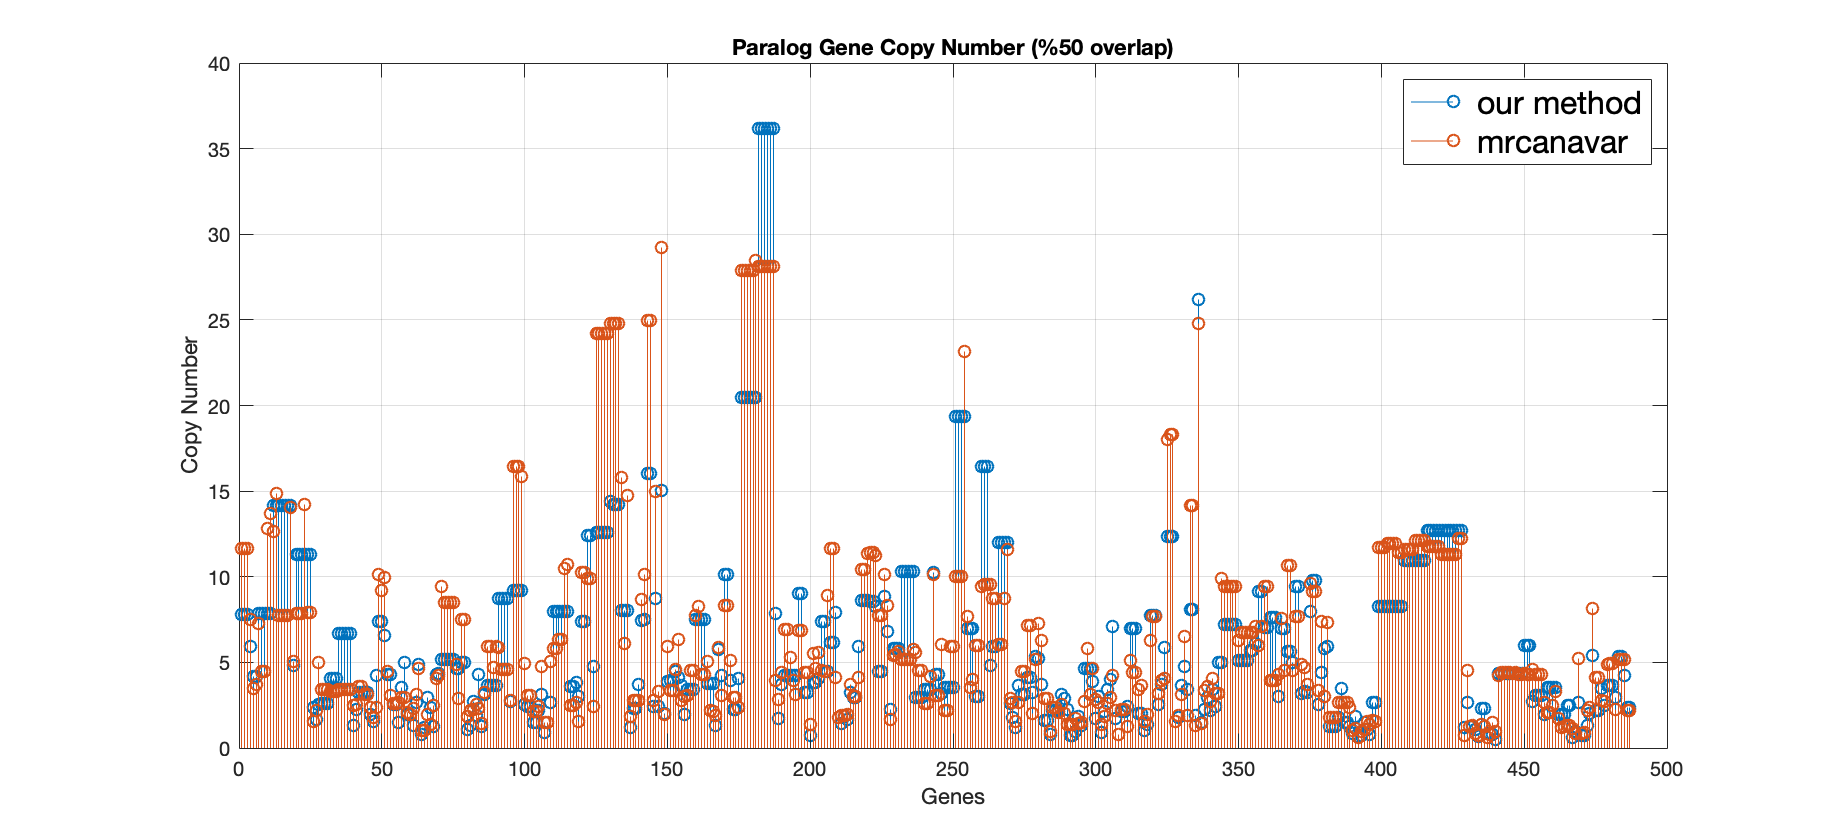
\includegraphics[scale=0.30]{images/42/figure3.png}\label{42overlap50}}
    \caption{Absolute copy numbers of genes showing \%50 overlapping by both methods}
    \label{overlap50}
\end{sidewaysfigure}

\begin{table}[]
\centering
\begin{tabular}{lllll}
\hline
\multicolumn{2}{l}{}                                                                         & \textbf{\textless{}10} & \textbf{10-20} & \textbf{20+} \\ \hline
\multicolumn{1}{l|}{\multirow{2}{*}{\textbf{\%90 overlap}}} & \multicolumn{1}{l|}{NA12878}   & 92                        & 6              & 0            \\ \cline{2-5} 
\multicolumn{1}{l|}{}                                       & \multicolumn{1}{l|}{42S291210} & 71                        & 19             & 1            \\ \hline
\multicolumn{1}{l|}{\multirow{2}{*}{\textbf{\%75 overlap}}} & \multicolumn{1}{l|}{NA12878}   & 224                       & 30             & 12           \\ \cline{2-5} 
\multicolumn{1}{l|}{}                                       & \multicolumn{1}{l|}{42S291210} & 177                       & 34             & 8            \\ \hline
\multicolumn{1}{l|}{\multirow{2}{*}{\textbf{\%50 overlap}}} & \multicolumn{1}{l|}{NA12878}   & 501                       & 88             & 36           \\ \cline{2-5} 
\multicolumn{1}{l|}{}                                       & \multicolumn{1}{l|}{42S291210} & 388                       & 73             & 26           \\ \hline
\multicolumn{1}{l|}{\multirow{2}{*}{\textbf{\%25 overlap}}} & \multicolumn{1}{l|}{NA12878}   & 778                       & 135            & 48           \\ \cline{2-5} 
\multicolumn{1}{l|}{}                                       & \multicolumn{1}{l|}{42S291210} & 561                       & 142            & 66           \\ \hline
\end{tabular}
\caption{Comparison of methods according to copy number values. The rows indicate the overlapping percentage and the columns indicate absolute copy numbers. Genes having higher absolute copy number often have lower overlapping.}
\label{overlapVScnvNo}
\end{table}